% This is samplepaper.tex, a sample chapter demonstrating the
% LLNCS macro package for Springer Computer Science proceedings;
% Version 2.20 of 2017/10/04
%
\documentclass[runningheads]{llncs}
%
% \usepackage[lofdepth,lotdepth]{subfig}
\usepackage{graphicx}
\usepackage{subcaption}
\usepackage{caption}
\usepackage{float}
% \usepackage{subfigure}
\usepackage{algorithm}
\usepackage[noend]{algpseudocode}
\usepackage{listings,chngcntr}
\usepackage{xcolor} % for setting colors
\usepackage{hyperref}
\usepackage{multirow}
\usepackage{array}
\usepackage{calc}
\newcommand{\algorithmautorefname}{Algorithm}
\newcommand{\definitionautorefname}{Definition}
\newcommand*\Let[2]{\State #1 $\gets$ #2}
\newfloat{algorithm}{t}{lop}

\renewcommand\UrlFont{\color{blue}\rmfamily}

% \usepackage[labelfont=bf,font=small,skip=5pt]{caption}
% \usepackage{subcaption}


% set the default code style
\lstset{
    basicstyle=\footnotesize,
    frame=tb, % draw a frame at the top and bottom of the code block
    tabsize=2, % tab space width
    showstringspaces=false, % don't mark spaces in strings
    numbers=left, % display line numbers on the left
    commentstyle=\color{green}, % comment color
    keywordstyle=\color{blue}, % keyword color
    stringstyle=\color{red} % string color
}
\lstdefinestyle{customc}{
%   belowcaptionskip=1\baselineskip,
  breaklines=true,
  frame=L,
  xleftmargin=\parindent,
  language=C,
  showstringspaces=false,
  basicstyle=\scriptsize\ttfamily,
  keywordstyle=\bfseries\color{green!40!black},
  commentstyle=\itshape\color{purple!40!black},
  identifierstyle=\color{blue},
  stringstyle=\color{orange},
}
\lstdefinestyle{customcnonum}{
%   belowcaptionskip=1\baselineskip,
  breaklines=true,
  frame=L,
  xleftmargin=\parindent,
  language=C,
  numbers=none,
  showstringspaces=false,
  basicstyle=\tiny\ttfamily,
  keywordstyle=\bfseries\color{green!40!black},
  commentstyle=\itshape\color{purple!40!black},
  identifierstyle=\color{blue},
  stringstyle=\color{orange},
}

% Used for displaying a sample figure. If possible, figure files should
% be included in EPS format.
%
% If you use the hyperref package, please uncomment the following line
% to display URLs in blue roman font according to Springer's eBook style:
% \renewcommand\UrlFont{\color{blue}\rmfamily}

\begin{document}
\counterwithin{lstlisting}{section}

%
\title{OmpSan: Static Verification of OpenMP's Data Mapping constructs}
%
%\titlerunning{Abbreviated paper title}
% If the paper title is too long for the running head, you can set
% an abbreviated paper title here
%
\author{Prithayan Barua\inst{1} \and
Jun Shirako\inst{1} \and
Whitney Tsang\inst{2} \and
Jeeva Paudel\inst{2} \and
Wang Chen\inst{2} \and
Vivek Sarkar\inst{1}
}
%
\authorrunning{Barua, P et al.}
% First names are abbreviated in the running head.
% If there are more than two authors, 'et al.' is used.
%
\institute{Georgia Institute of Technology \and
IBM Toronto Laboratory
}

\maketitle              % typeset the header of the contribution
%
\begin{abstract}
OpenMP has made it convenient to port an existing application from CPU to heterogeneous systems like GPUs. Starting from 4.5 standard, target offloading features can be used to offload individual kernels to the GPU and other devices. 
Several users have noted that one of the most challenging and error-prone tasks is the memory management for the device offloading. 
% Typically developers spend majority of their time, understanding
% the correct usage and performance implications 
% of the target \texttt{map} clause.  

In this paper, we present a static analysis tool, 
OmpSan, a code sanitizer, that helps the developers understand the 
correct usage and performance implications of
the target \texttt{map} clause. We present several 
case-studies to show the effectiveness of our powerful analysis.
OmpSan can detect bugs resulting from incorrect usage of 
\texttt{map} clause, and also report diagnostic information
 and simple fixes for the bug.


\keywords{OpenMP Offloading \and OpenMP Target Data Mapping \and LLVM \and Memory Management
 \and Static Analysis \and Verification \and Debugging}
\end{abstract}
%
%
%
\section{Introduction}
\label{s1}
% /* Notes
% (TODO: the address on the deice is diferent)
% Alloc: just allocate on device, uninitialized
% to: map to device before execution
% from:  map from device after execution
% tofrom: map to and from
% https://www.appentra.com/about-us/
% */
Open Multi-Processing (OpenMP) is a widely used directive-based parallel programming model
that  supports offloading computations from hosts to accelerator devices such as GPUs. 
% which offers accelerator programming and supports heterogeneous
% computing systems with host CPUs and device accelerators (currently
% GPUs and FPGAs) from version 4.0 onwards.  
Notable accelerator-related features 
in OpenMP include unstructured data
mapping, asynchronous execution, and runtime routines for device
memory management. 
% \vspace{-10pt}
\subsubsection{OMP Target offloading and Data mapping}
OMP offers the \texttt{omp target} directive 
for offloading computations to devices and the \texttt{omp target data}
directive for mapping data across the host and the corresponding
device data environment.
% is used to generate a target 
% task that can be offloaded to a device, and also to map variables 
% to the device data environment. 
% The \textit{omp target data} directive explicitly maps variables 
% from a host environment to a device data environment.
On heterogeneous systems, managing the movement of data between the host and the device can be challenging, and is often a major source of performance and correctness bugs. 
In the OpenMP accelerator model, 
% hosts and devices have their own memory space – i.e., data environments – and 
data movement between device and host 
is supported either explicitly via the use of a \texttt{map} clause 
or, implicitly through default data-mapping rules. 
The optimal, or even correct, specification of map clauses can be non-trivial and error-prone because it requires users to reason about the complex dataflow analysis. 
To ensure that the map clauses are correct, the OpenMP programmers 
need to make sure that variables that are defined in one data environments and used in another data environments are mapped accordingly across 
the different device and host data environments. 
Given a data map construct, its semantics depends on all the previous usages of the map construct.
Therefore, dataflow analysis of map clauses is necessarily 
context-sensitive since the entire call sequence leading up to a specific 
map construct can impact its behavior.
% To ensure that the map clauses are correct, OpenMP programmers 
% need to identify statements 
% that define variables involved in target clauses, and
% each definition of such a variable to all the uses that can be 
% reached by it in the program.
% Given a data map construct, its semantics depends on all the previous usages of the map construct.
% Therefore, dataflow analysis of map clauses is necessarily 
% context-sensitive since the entire call sequence leading up to a specific 
% map construct can impact its behavior.
% 
% Therefore, it is context sensitive and the entire call sequence leading up to the construct impacts its behavior.
% On heterogeneous systems, managing the 
% movement of data between the host and the 
% the data movement between host and device is
% a common performance and energy efficiency bottleneck, as well as a
% major source of performance and correctness bugs.  In the OpenMP
% accelerator model, host and device have their own memory space --
% i.e., data environment -- and the data movement is supported by the
% explicit data copy via \texttt{map} clause or, implicitly through 
% default \texttt{map} rules.
% The optimal, or even
% correct specification of \texttt{map} clause is non-trivial and 
% error-prone because it requires element-wise dataflow analysis to
% identify the statements/instructions that define the value at given
% program points and variables/array elements.
% Even given an existing application that uses the 
% target offloading feature, understanding the data mapping 
% behavior is nontrivial. 
% Given a data map construct, its semantics depends on all the previous 
% usages of the map construct. Therefore, it is context sensitive and 
% the entire call sequence leading up to the construct impacts its 
% behavior.
\subsection{OpenMP 5.0 Map Semantics}
\autoref{mapSemantics} shows a schematic illustration 
of the set of rules used when mapping 
a host variable to the corresponding list item 
in the device data environment, as specified 
in the OpenMP 5.0 standard. The rest of this paper 
 assumes that the accelerator device is a GPU, and that mapping 
a variable from host to device introduces a host-to-device memory copy, 
and vice-versa. 
However, the bugs that we identify reflect errors in the OpenMP 
code regardless of the target device. 

The different map types that OpenMP 5.0 supports are, 
\begin{itemize}
\vspace{-5pt}
 \item \texttt{alloc}: allocate on device, uninitialized
 \item \texttt{to}: map to device before kernel execution, (host-device memory copy)
 \item \texttt{from}:  map from device after kernel execution (device-host memory copy)
 \item \texttt{tofrom}: copy in and copy out the variable at the entry and exit of the device environment  
\end{itemize}
\vspace{-9pt}
%% The default map type for arrays is \textit{tofrom}, 
%% % that is copy in and copy out the array at the entry and exit of 
%% % the device enviro nment. 
%% while the default for scalars
%% is \textit{firstprivate}, that is the only copy the value of the 
%% scalar at the entry to the device environment.
Arrays are implicitly mapped as \texttt{tofrom}, while scalars are firstprivate 
 in the target region implicitly, {\em i.e.,} the value of the scalar on the host
is copied to the corresponding item on the device only at the entry to the device
environment.
\begin{figure}[h!]
% \hspace{-80pt}
% \vspace{-20pt}
\begin{subfigure}[b]{1\textwidth}
\centering
    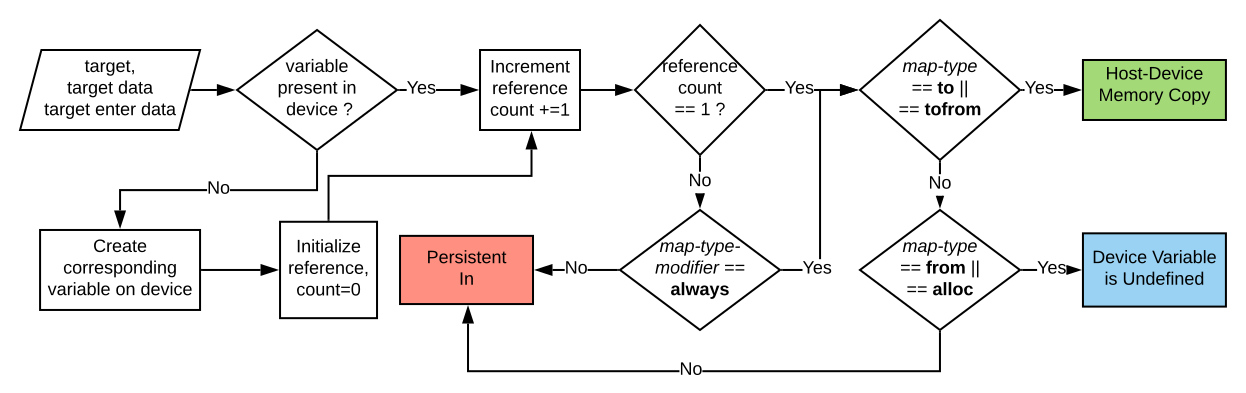
\includegraphics[scale=0.6]{images/data-enter.png}
  \caption{Flowchart for Enter Device Environment}
    \label{host-device-flowchart}    
  \end{subfigure} 
  
%   \hspace{20pt}
  \begin{subfigure}[b]{1\textwidth}
  \centering
    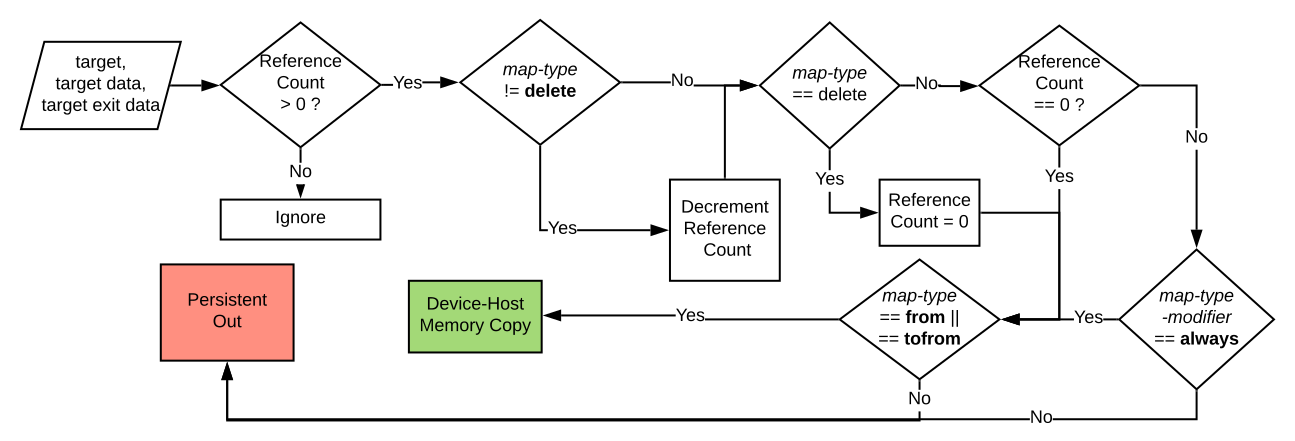
\includegraphics[scale=0.6]{images/data-exit.png}
    \caption{Flowchart for Exit Device Environment}
    \label{device-host-flowchart}    
  \end{subfigure}
  \caption{Flowcharts to show how to interpret the map clause}    
  \label{mapSemantics}
%   \vspace*{-10pt}
\vspace{-10pt}
\end{figure} 
% The OpenMP 5.0 specification specifies the semantics of the \textit{map}
% clause, and \autoref{mapSemantics} illustrates how the spec 
% interprets the data map constructs. 
% The flowchart also motivates our argument that understanding the \textit{map} clause is not trivial, it 
%  shows the complex set of rules defined in the OpenMP 5.0 spec, 
% that is used to determine how to map a  host variable to the corresponding list item in the device data environment.
% We make a simplifying assumption that the CPU host is the current 
% task's data environment and the device is a GPU, and hence the mapping from the host to the device
% refers to the Device-Host and Host-device memory copy.
As \autoref{mapSemantics} shows, OpenMP 5.0 specification uses the reference count of a variable, to decide when to introduce 
a device/host memory copy. The host to device memory copy is 
introduced only when the reference count is incremented from 0 to 1 and the \texttt{to} attribute is present. 
Then the reference count is incremented every time a 
new device map environment is created. 
The reference count is decremented on encountering a \texttt{from} or \texttt{release} 
attribute, while exiting the data environment. 
Finally, when the reference count is decremented to zero from 1, and the 
\texttt{from} attribute is present, 
the variable is mapped back to the host from the device.
% \autoref{statemachine} shows an example state machine, 
% to decide when to insert the memory copies.
% \begin{figure}
% %  \hspace*{-30pt}
%     \includegraphics[scale=0.6]{images/statemachine.png}
%     \caption{State Machine for inserting Host/Device Memory Copies } \label{statemachine}
% \end{figure}
\vspace{-10pt}
\subsection{The Problem}
For target offloading, the map clause is used to map variables from a 
task's data environment to the corresponding variable in the device 
data environment. Incorrect data map clauses can result in 
usage of 
stale data in either host or device data environment, 
which may result in the following kinds of issues, 
% Now if a map clause is used incorrectly, 
% then the read of a variable can return stale data.

\begin{itemize}
 \item The variable on the device data environment, does not contain 
 the updated values of its original variable.
 \item The original variable was not updated with the latest value of 
 the device environment variable.
\end{itemize}


\subsection{Our Solution}
% \vspace{-50pt}
We propose a static analysis 
tool called OMPSan to perform OpenMP code ``sanitization''.
OMPSan is a compile-time tool, which statically verifies  
the correctness of the  data mapping constructs based on a dataflow analysis.
The key principle guiding our approach is that: {\em an OpenMP program is expected to yield the same result when enabling
or disabling OpenMP constructs}.
% this issue as first-aid error detection, we propose a
% compile-time approach based on dataflow analysis. 
% The key principle guiding our error detection approach is that
% ``A user program yields the same result when enabling or disabling
% OpenMP constructs''.
% \footnote{With the exception of privatization clauses, which is unrelated to our goal, and beyond the scope of this work}.
Our approach detects errors by comparing the 
dataflow information (reaching definitions via
LLVM's memory SSA representation \cite{llvm-memoryssa-url}) 
between the OpenMP and baseline code.  We developed an
LLVM-based implementation of our approach and evaluated its
effectiveness using several case studies.
Our specific contributions include:
\begin{itemize}
% \vspace{-3pt}
\item an algorithm to analyze OpenMP runtime library calls inserted by Clang in the LLVM IR, to infer the host/device memory copies. We expect 
that this algorithm will have applications beyond our OMPSan tool. 
% according to OpenMP 5.0 semantics
\item a static analysis technique to validate if the host/device memory copies respect the original memory def-use relations. 
% \item Reporting error/warnings on usage of data mapping constructs 
% on given user programs
\item diagnostic information for users to understand how the map clause affects the 
host and device data environment. 
\end{itemize}
Even though our algorithm is based on clang OpenMP implementation, 
it can very easily be applied to other approaches like using directives 
to delay the OpenMP lowering to a later LLVM pass.  
% \vspace{-10pt}
The paper is organized as follows. 
\autoref{s2} provides motivating examples to describe 
the common issues and difficulties in using 
OpenMP's \textit{data map} construct. 
\autoref{s03} provides the background information 
that we use in our analysis.
\autoref{s3} presents an overview of our approach to validate 
the usage of data mapping constructs. 
\autoref{s4} presents the LLVM implementation details, and 
\autoref{s5} presents the evaluation and some case studies. 
\autoref{limitation} also lists some of the limitations of 
our tool, some of them common to any static analysis.  
% \vspace{-20pt}
% According to the OpenMP 5.0 semantics, the \texttt{target}, 
% \texttt{target data}, and the \texttt{target enter data} 
% constructs maps host variables to a device data environment. Essentially 
% for the GPU, it inserts host-device and device-host memory copies. 
% The \texttt{map} clause is used to specify how a variable is mapped 
% from the host to the device environment.


\section{Motivating Examples}
\label{s2}
To motivate the utility and applicability of OmpSan,
we discuss 3 potential errors in user code arising from 
improper usage of the data mapping constructs.
% We discuss potential errors in the user code arising 
% from improper usage of the data mapping constructs, 
% and illustrate how easy it is to incorrectly use the map 
% construct. 
% The accompanying examples motivate the utility and applicability of our proposed analysis and the tool OMPSan.

% We show several common pitfalls of the OpenMP data map construct, 
% and illustrate how easy it is to incorrectly use the map 
% construct, and thus motivate the need for our tool.
\vspace{-10pt}
\subsection{Default Scalar Mapping}
In Our first example, \autoref{incorrectegs1},  
 the definition of ``sum'' on line 5 does not reach line 6,
since the ``sum'' does not have an explicit mapping and the default
map for scalars is ``firstprivate''. 
As \autoref{incorrectegs-fix1} shows, an explicit map clause 
is essential to specify the 
copy in and copy out of the scalar ``sum'' from device.

\begin{minipage}{.4\textwidth}
\begin{lstlisting}[style=customc, frame=tlrb, caption={Default scalar map}, label=incorrectegs1]
int A[N], sum=0, i;
#pragma omp target
#pragma omp teams distribute parallel for reduction(+:sum)
  for(i=0; i<N; i++) 
    sum += A[i];
  printf("\n%d",sum);
\end{lstlisting}
\end{minipage}\hfil
\begin{minipage}{.4\textwidth}
\begin{lstlisting}[style=customc, frame=tlrb, caption={Explicit map}, label=incorrectegs-fix1]
int A[N], sum=0;
#pragma omp target map(tofrom:sum)
#pragma omp teams distribute parallel for reduction(+:sum)
  for( int i=0; i<N; i++) 
    sum += A[i];
  printf("\n%d",sum);
\end{lstlisting}
\end{minipage}

\subsection{Reference Count Issues}
\subsubsection{Example 1}
\autoref{incorrectegs3} shows an example of data-mapping 
attributes across different data environments.
The array ``B'', is specified as ``alloc'' in the first 
data environment. According to OpenMP 4.5 (\autoref{mapSemantics}) 
exiting a data environment where the variable was mapped as ``alloc'' does not decrement the reference count, and a variable is mapped 
back from device to host only if the reference count is decremented to 0. 
We can track the reference count for ``B'' is as follows, 
\begin{itemize}
% \vspace*{-10pt}
 \item Line 5, reference count = 1
 \item Line 6, enter data environment, reference count = 2
 \item Line 8, exit data environment ``alloc'', reference count = 2
 \item Line 9, exit data environment ``from'', reference count =1
 \item Line 12 accesses stale data of ``B'', 
 since it was not mapped back to host
\end{itemize}
% 
% variable is set to 1 at line 5, as we enter a new 
% data environment. Then we enter another 
% data environment at line 6, which increments the reference count 
% to 2. But as we exit the environment at line 8, 
% because of the ``alloc'' attribute, the reference count of variable ``B'' 
% is not decremented, so at line 8, reference count is 8, and line 9
% ends the data environment, and has a ``from'' attribute
% which decrements the reference count to 1. Since the reference count 
% is not zero, array ``B'' is not mapped back to host.
% By specifying the ``from'' attribute on the map clause for the 
% variable ``B'' on line 9, 
% the user would hope to see the updated value of B from the device 
% to be available on the host as well. 
% However, such an expectation would be incorrect, and 
% easily missed by the user owing to reference-count rules
% that guide data copy-in/out outcomes. As such corresponding 
% value of ``B'' on host is not updated.
As \autoref{incorrectegs-fix3} shows, replacing ``alloc'' 
with ``from'' on line 6, will update the host version of ``B'' 
on exit of the map region at line 9.

(Note: This is no longer a bug in OpenMP 5.0, since even ``alloc'' 
 decrements the reference counter)

\begin{minipage}{.4\textwidth}
\begin{lstlisting}[style=customc, frame=tlrb, caption={Usage of alloc}, label=incorrectegs3]
int A[10], B[10];
for (int i =0 ; i < 10 ; i++)
    A[i] = i;

#pragma omp target enter data map(to:A[0:10]) map(alloc:B[0:10])
#pragma omp target map(alloc:B[0:10])
for (int i = 0 ; i < 10; i++)
    B[i] = A[i];
#pragma omp target exit data map(from:B[0:10])

for (int i = 0 ; i < 10; i++)
    printf("%d",B[i]);
\end{lstlisting}
\end{minipage}\hfil
\begin{minipage}{.4\textwidth}
\begin{lstlisting}[style=customc, frame=tlrb, caption={Usage of from}, label=incorrectegs-fix3]
int A[10], B[10];
for (int i =0 ; i < 10 ; i++)
    A[i] = i;

#pragma omp target enter data map(to:A[0:10]) map(alloc:B[0:10])
#pragma omp target map(from:B[0:10]) 
for (int i = 0 ; i < 10; i++)
    B[i] = A[i];
#pragma omp target exit data map(from:B[0:10])

for (int i = 0 ; i < 10; i++)
    printf("%d",B[i]);
\end{lstlisting}
\end{minipage}

This example shows the difficulty in interpreting an 
independent map construct. 
Especially when we are dealing with the global variables 
and map clauses across different functions, 
maybe even in different files, 
it becomes nearly impossible to understand 
and identify potential incorrect usages of 
the map construct. 
Our static analysis tool can report diagnostics and errors with possible fixes to help the developers in using the data mapping clauses.
% 
% 
% can not only 
% error out on such issues, 
% but also the show debug information 
% to help understand how each map construct 
% is interpreted based on its context.
\subsubsection{Example 2} 
\autoref{incorrectegs2} shows another example of a reference count issue. 
% reference count, user might not get the expected behavior. 
The line, 9 which executes on the host, does not read
the value of ``A'' that was updated on device at line 7. 
This is again because of the ``from'' clause on line 5, increments 
the reference count to 2 on entry, and back to 1 on exit, hence 
after line 7, ``A'' is not copied out to host.
\autoref{incorrectegs-fix2} shows the usage of ``update'' 
to force the copy-out, and read the expected updated ``A'' on line 11.
% incorrect usage of map clause. 
% The user declared the target data environment on line 3, with ``A'' mapped as ``from''. According to the OpenMP 4.5 semantics, the map clause on line 3, 
% will instantiate an uninitialized version of array ``A'' on device, 
% and also associate a reference count with it. The reference count will 
% be set to 1, after the  line 3. Now the map clause on the ``target'' 
% construct, at line 5, will have no affect on the device copy of ``A'', but 
% still it will increment the reference count to 2 at line 5. 
% At the exit of the offloaded loop, after line 7, the reference count 
% is 2, hence the ``from'' clause on line 5 will not have any affect, 
% other than decrementing the reference count to 1. 
% Now the line 9, that is executed on the host, will not 
% be reading the updated version of ``A'' from the device, line 7, 
% because ``A'' was not mapped back to the host after line 7.
% On exit of the data map region at line 10, the reference count is 
% decremented to 0, and only then the device copy of ``A'' is 
% mapped back and copied to the host. This is because of the 
% ``from'' map attribute on line 3. In this example, ``from'' 
% attribute on line 5, has no affect. 
% To fix this issue, we need to use the update clause as shown in 
% \autoref{incorrectegs-fix2}.

\begin{minipage}{.4\textwidth}
\begin{lstlisting}[style=customc, frame=tlrb,  caption={Reference Count}, label=incorrectegs2]
define N 100                                                                                            
int A[N], sum=0;
#pragma omp target data map(from:A[0:N]) 
  {
    #pragma omp target map(from:A[0:N])
    for(int i=0; i<N; i++) 
      A[i]=i;
    for(int i=0; i<N; i++) 
      sum += A[i];
  }
\end{lstlisting}
\end{minipage}\hfil
\begin{minipage}{.4\textwidth}
\begin{lstlisting}[style=customc, frame=tlrb, caption={Update Clause}, label=incorrectegs-fix2]

define N 100                                                                                            
int A[N], sum=0;
#pragma omp target data map(from:A[0:N]) 
  {
    #pragma omp target map(from:A[0:N])
    for(int i=0; i<N; i++) 
      A[i]=i;
    #pragma omp target update from(A[0:N])  
    for(int i=0; i<N; i++) 
      sum += A[i];
  }
\end{lstlisting}
\end{minipage}
% In the next section, we will introduce our static analysis tool, 
% which can identify such issues with the incorrect/unexpected 
% usage of OpenMP data mapping constructs. 
% Assuming the correct/expected
% behavior is same as when executing the OpenMP program by ignoring all the 
% OpenMP constructs.
% Lets look at an example to motivate that determining when to insert the
% memory copies is non-trivial and can result in incorrect programs, 
% if the programmer does not understand the OpenMP spec precisely. 
% \autoref{datamapping1} shows an example of incorrect usage of the openmp data mapping clause. 
% On line 4, the map clause, specifies \textit{tofrom}, hence at the entry and 
% exit of the omp region, host-device and device-host memory copy is introduced. 
% That is, a new device copy for the variable $sum$ is made at line   4, and 
% the host $sum$ is copied to the device $sum$. Line 6, increments the value to 1. 
% Line 7, where the region ends, copies back the device $sum$ to host $sum$, and hence
% line 8 prints the correct value of $sum$. Again Line 9, has the map clause \textit{to}, 
% which copies the host $sum$ to device $sum$ on line 10, but since \textit{from} is missing
% fromt he clause, the host copy is not updated on line 12, since the device to host memory copy
% is not present. Since, the host does not access, $sum$ on line 13, this is a valid behaviour. 
% But again on line 14, \textit{tofrom} maptype is used, but this time, since the $sum$ 
% was already present on the device, a host device memory copy is not inserted. Also, 
% since the reference count for $sum$ on device is now 2, and the \textit{from} maptype 
% only decrements the reference count to 1, the device-host copy is also not inserted on line 17. 
% This is a common mistake user can make, if he does not carefully follow the OpenMP 4.5 specs.
% 
% \begin{lstlisting}[style=customc, caption={data map clause}, label=datamapping1]
% int main()
% {
%     int sum = 0 ;
%     #pragma omp target data map (tofrom:sum)
%     {  /*H->D*/
%         sum++;  /* sum = 1 */
%     } /*D->H*/
%     printf("%d",sum); /* 1 */
%     #pragma omp target data map (to:sum)  
%     {  /*H->D*/
%         sum++;  /* sum = 2 */
%     }    
%     /* printf("%d",sum);  1 */
%     #pragma omp target data map (tofrom:sum) 
%     {
%         sum++;  /* sum = 3 */  
%     } 
%     printf("%d",sum); /* 3 */
%     return 0;
% }
% \end{lstlisting}


% \begin{lstlisting}[style=customc, caption={data map clause}, label=datamapping1]
%  static void init_ui(int d1, int d2, int d3)
% {
%   int i, j, k;
% 
% #pragma omp target map (alloc: u0_real,u0_imag,u1_real,u1_imag,twiddle)                                                                                                                                            
% //#pragma omp target update to(u0_real,u0_imag,u1_real,u1_imag,twiddle)
%   {
% //#pragma omp target 
% #pragma omp teams distribute 
%     for (k = 0; k < d3; k++) {
% #pragma omp parallel for 
%       for (j = 0; j < d2; j++) {
%         for (i = 0; i < d1; i++) {
%           u0_real[k*d2*(d1+1) + j*(d1+1) + i] = 0.0; 
%           u0_imag[k*d2*(d1+1) + j*(d1+1) + i] = 0.0; 
%           u1_real[k*d2*(d1+1) + j*(d1+1) + i] = 0.0; 
%           u1_imag[k*d2*(d1+1) + j*(d1+1) + i] = 0.0; 
%           twiddle[k*d2*(d1+1) + j*(d1+1) + i] = 0.0; 
%         }
%       }    
%     }    
%   }
% }
% static void evolve(int d1, int d2, int d3)
% {
%   int i, j, k;
% #pragma omp target map (alloc: u0_real,u0_imag,u1_real,u1_imag,twiddle)
%   {
% #pragma omp teams distribute
%     for (k = 0; k < d3; k++) {
% #pragma omp parallel for
%       for (j = 0; j < d2; j++) {
% #pragma omp simd
%         for (i = 0; i < d1; i++) {
%           u0_real[k*d2*(d1+1) + j*(d1+1) + i] = u0_real[k*d2*(d1+1) + j*(d1+1) + i]*twiddle[k*d2*(d1+1) + j*(d1+1) + i];
%           u0_imag[k*d2*(d1+1) + j*(d1+1) + i] = u0_imag[k*d2*(d1+1) + j*(d1+1) + i] *twiddle[k*d2*(d1+1) + j*(d1+1) + i];
%           u1_real[k*d2*(d1+1) + j*(d1+1) + i] = u0_real[k*d2*(d1+1) + j*(d1+1) + i];
%           u1_imag[k*d2*(d1+1) + j*(d1+1) + i] = u0_imag[k*d2*(d1+1) + j*(d1+1) + i];
%         }
%       }
%     }
%   }
% }
% ft.c:#pragma omp target map (alloc: u0_real,u0_imag,u1_real,u1_imag,twiddle)
% ft.c:#pragma omp target map (alloc: u0_real,u0_imag,u1_real,u1_imag,twiddle)
% ft.c:#pragma omp target map(alloc:twiddle)
% ft.c:#pragma omp target map(alloc: u_real,u_imag) 
% ft.c:#pragma omp target map(alloc: u_real,u_imag) map(to:t)
% ft.c:#pragma omp target map(alloc: gty1_real,gty1_imag,gty2_real,gty2_imag, u1_real, u1_imag)\
% ft.c:#pragma omp target map ( alloc: u1_real, u1_imag, u_real,u_imag)\
% ft.c://#pragma omp target map(alloc: gty1_real,gty1_imag,gty2_real,gty2_imag,\
% ft.c://#pragma omp target map(alloc: gty1_real,gty1_imag,gty2_real,gty2_imag,\
% ft.c:#pragma omp target map (alloc: u1_real, u1_imag, u_real,u_imag, gty1_real, gty1_imag, gty2_real, gty2_imag) 
% ft.c://#pragma omp target map(alloc: gty1_real,gty1_imag,gty2_real,gty2_imag,\
% ft.c:#pragma omp target map (alloc: u1_real, u1_imag, u_real,u_imag, gty1_real, gty1_imag, gty2_real, gty2_imag) 
% ft.c:#pragma omp target map (alloc: u1_real, u1_imag) map(tofrom: temp1, temp2)
% \end{lstlisting}

\section{Background}
\label{s03}
\subsection{Memory SSA} Our analysis is based on the LLVM 
 Memory SSA \cite{llvm-memoryssa-url} \cite{Novillo_memoryssa}, 
 which is an imprecise 
implementation of Array SSA\cite{Knobe:1998:ASF:268946.268956}.
% Memory SSA captures the 
% use-def chains for every memory access in the program. 
We construct the def-use chains for each array variable, 
based on the Memory SSA. 
% The store instruction 
% corresponds to the definition, and load instruction corresponds 
% to memory use, and Memory Phi nodes merge the \textit{may} reach 
% definitions. 
LLVM Memory SSA is a virtual IR, where every definition and phi 
node creates a new version of memory, which are numbered.
The Memory SSA IR has the following kinds of instructions/nodes, 
\begin{itemize}
% \vspace{-10pt}
 \item $INIT$, a special node to signify uninitialized or live on 
 entry definitions
 \item $MemoryDef(N)$, corresponds to a memory store
 instruction, and where $N$ identifies the last write that this 
 definition clobbers
 \item $MemoryUse(N)$, where N is the reaching definition, that 
 this node uses
 \item $MemPhi(N_1,N_2,...)$, where $N_i$ is one of the  
 may reaching definitions
\end{itemize}
We make the following simplifying assumptions, to keep the analysis
tractable
\begin{itemize}
% \vspace{-8pt}
 \item Given an array variable we can find all the  corresponding
 load and store instructions.
 \item A $MemoryDef$ node, clobbers the entire array associated 
 with its store instruction.
 \item $MemoryPhi$ nodes are inserted only at the entry 
 of basic blocks, which have more than one $MemoryDef$s that can 
 flow into the basic block.
 \item We are concerned with only those array variables that 
 are mapped to a target offload region. 
\end{itemize}
% \vspace{-16pt}
\subsection{Scalar Evolution Analysis}\vspace{-5pt}
LLVM's Scalar Evolution (SCEV) is a very powerful technique
that can be used to analyze the change in 
the value of scalar variables over iterations of a loop, as chain 
of recurences. 
% We can use the SCEV analysis to represent the loop induction variables 
% as chain of recurrences. 
% This mathematical representation 
% can then be used to analyze the variables used to index into memory 
% operations. 
Then it can be used to symbolically evaluate the 
minimum and maximum value of every array index expression. 
% In case the SCEV analysis fails to model an expression, 
% we over approximate the range of the array indices to the 
% maximum dimensions of the array variable. 
\autoref{s4} has details 
of how we implement the analysis and handle different cases. 

\section{Our Approach}
\label{s3}
% \begin{minipage}{.45\textwidth}
% \begin{lstlisting}[style=customc, frame=tlrb, caption={Example Code 1}, label=memorySSA-example-1]
% 
% L1: for ( i =0 ; i < 100 ; i++) {
%         S1: A[i] = 0;
%     }
% #pragma omp target enter data map(to:A[0:50], alloc:C[0:100])
% #pragma omp target
% L2: for (i=0; i < 100; i++ ) {
%         S2: t = A[i] ;
%         S3 C[i] = t; 
%     }    
% #pragma omp target exit data map( release:C[0:100])
% L3: for (i=0; i < 100; i++) {
%         S4: print(C[i])
%     }
% \end{lstlisting}
% \end{minipage}
% In this work, we assume that variables
% that have corresponding list items across host and device 
% boundary or across different data environment boundaries 
% on the device need to be updated at the edge of such boundaries. 
% Typically this assumption reflects the practical use-case of the variables. 
OmpSan assumes certain practical use cases, for example, in \autoref{incorrectegs3}, a user would expect the updated 
value of ``B'' after the second data environment on line 12. 
Having said that, a skilled ninja programmer 
may very well expect ``B'' to remain stale, because of his knowledge 
and understanding of the complexities of data mapping rules. 
Our analysis and error/warning reports from this work are 
intended only for the former case.

Here we first outline the key steps of our approach with the algorithm
and exemplify it with a concrete example
to illustrate the algorithm in action.
\vspace{-10pt}
\subsection{Algorithm}
\begin{algorithm}[!htbp]
    \caption{Overview of Data Mapping Analysis}
    \label{dataMapAnalysisAlgo}
    \begin{algorithmic}[1]
        \small 
    \Function{$\textsc{DataMapAnalysis}$}{$Module$}
        \State $MappedArrayVars=\phi$
        \For{$ArrayVar \in MapClauses$}
            \State $MappedArrayVars = MappedArrayVars \cup ArrayVar$
        \EndFor
        \State \texttt{ConstructArraySSA}($Module, MappedArrayVars$)
        \State \texttt{InterpretTargetClauses}($Module, MappedArrayVars$)
        \State \texttt{ValidateDataMap}($MappedArrayVars$)
    \EndFunction
    \Function{$\textsc{ConstructArraySSA}$}{$Module, MappedArrayVars$}
%         \State $MappedArrayVars=\phi$
%         \For{$ArrayVar \in MapClauses$}
%             \State $MappedArrayVars = MappedArrayVars \cup ArrayVar$
%         \EndFor
        \For {$MemoryAccess \in Module$}            
            \State $ArrayVar$ = \texttt{getArrayVar}($MemoryAccess$)
            \If{ 
                $ArrayVar \in MappedArrayVars$ }
            \If { $MemoryAccess  \in OMP\_targetOffload\_Region$}
                \State $targetNode = true$
                \Comment{If Memory Access on device}
            \Else
                \State $targetNode = false$
                \Comment{If Memory Access on host}
            \EndIf
            \State $Range= $ \texttt{SCEVGetMinMax}$(MemoryAccess)$
            \State $underConstruction$= \texttt{GetArraySSA}$(ArrayVar)$
            
            \State \Comment{could be null or incomplete}
            
            \State \texttt{InsertNodeArraySSA}($underConstruction$,$MemoryAccess, targetNode, range$ )
%             \Comment{Incrementally construct, by adding this access}
            \State  \Comment{Incrementally construct, by adding this access}            
            \EndIf 
        \EndFor
        \EndFunction
        \Function{$\textsc{InterpretTargetClauses}$}{$Module, MappedArrayVars$}
        \For {$ArrayVar \in MappedArrayVars$ }
            \State $ArraySSA =$ \texttt{GetArraySSA}($ArrayVar$)
            \For { \textbf{edge}, $(node, Successornode) \in $ ($ArraySSA$) }
%                 \State $node$ = $edge.from$
                \State $nodeIsTarget =$ \texttt{isTargetOffload}($node$)
                
                \State $succIsTarget =$ \texttt{isTargetOffload}($Successornode$)
                \If { $nodeIsTarget \ != succIsTarget$}
                    \State \texttt{RemoveArraySSAEdge(                                                                                                                                                                                                                                                                                                                                                                                                                                                                                                                                                                                                                                                                                                                                                                                                                                                                                                                                                                                                                                                                                                                                                                                                                                                                                                                                                                                                                                                                                                                                                                                                                                                                                                                                                                                                                                                                                                                                                                                                                                                                                                                                                                                                                                                                                                                                                                                          $node$, $Successornode$ )}
                                        
                \EndIf                                                
            \EndFor 
        \EndFor 
        \For {$dataMap   \in dataMapClauses$}
            \State $hostNode$ = \texttt{getHostNode}($dataMap$)
            \State $deviceNode$ = \texttt{getDeviceNode}($dataMap$)
            \State $mapType =$ \texttt{getMapClauseType(}$ dataMap$)
                    \State \Comment{alloc/copyIn/copyOut/persistentIn/persistentOut}
                    \State \texttt{InsertDataMapEdge}($hostNode, deviceNode, 
                    mapType$)
        \EndFor
        \EndFunction
        \Function{$\textsc{ValidateDataMap}$}{$MappedArrayVars$}
        \For {$ArrayVar \in MappedArrayVars$ }
            \State $ArraySSA =$ \texttt{GetArraySSA}($ArrayVar$)
            \For { $memUse  \in $ \texttt{getMemoryUseNodes}($ArraySSA$)}
                \State $useRange$ = $\texttt{getReadRange(memUse)}$
                \State $clobberingAccess =$ \texttt{getClobberingAccess}$(ArraySSA, memUse)$
                \If { \texttt{isPartiallyReachable}($ArraySSA, 
                    clobberingAccess, memUse, useRange$) }
                    \State Report WARNING 
%                     \texttt{Report}($ArraySSA, 
%                     clobberingAccess, memUse, useRange$)                
                \ElsIf { \texttt{isNotReachable}($ArraySSA, 
                    clobberingAccess, memUse$) }
                    \State Report ERROR 
%                     \texttt{Report}($ArraySSA, 
%                     clobberingAccess, memUse, useRange$) 
                \EndIf
            \EndFor
        \EndFor    
        \EndFunction
    \end{algorithmic}
\end{algorithm}
The \autoref{dataMapAnalysisAlgo} shows an overview 
of the data map analysis. Firstly, we 
collect all the array variables used in the various
map clauses in the entire module. 
Then line 5, calls the function \texttt{ConstructArraySSA}, 
which constructs the array ssa for each of the mapped Array variables.
Then, we call the function, \texttt{InterpretTargetClauses}, 
which modifies the Array SSA graph, as per the map semantics of the 
program.
Then finally \texttt{ValidateDataMap} checks the 
reachability on the final graph, to validate 
the map clauses, and generates 
a diagnostic report with the warnings and errors.
% inline all user defined functions, and then use 
% the Memory SSA to construct the memory use-def chains, 
% for every array variable. After step 2, we get a graph for each
% memory array, with an edge from a $MemoryDef$
% or $MemPhi$ to the corresponding $MemoryUse$ or $MemPhi$ for the
% reaching definition relation. 
% Then we use the Scalar Evolution Analysis, to compute 
% the range of locations accessed by every memory reference.
% If the analysis fails to compute the range of locations 
% statically, then we over-approximate it to the 
% maximum size of the array.
% 
% Now we interpret
% the semantics of the \texttt{target} construct, 
% to classify the Memory SSA nodes, as executing on host or device.
% Since the device and host have a separate data environment, 
% they refer to different array variables. So in step 5, we remove the edges between host and device nodes. 
% Now according to the semantics of the \texttt{map} clause, 
% the host variables are mapped to the device variables, and 
% vice-versa. At any program point, when a 
% host variable is mapped to device, 
% we find its corresponding reaching definition, 
% and add a special edge from the host $MemoryDef$ or $MemPhi$, 
% to the $MemoryUse$ or $MemPhi$ on the device. 
% Similarly when mapping a device variable to host variable, 
% we add the edge between the corresponding definition on the device
% to the corresponding use on the host.
% In step 6, we also annotate the edges with the array sections 
% according to the \texttt{map} clause.
% 
% Finally, we report an error for every missing use-def 
% edge in our graph, since it indicates a mismatch
% between the sequential use-def relations and the OpenMp 
% reaching definitions. We report a warning, when an edge indicates
% that the array is partially mapped, and the $MemUse$
% could potentially access locations outside the mapped range.

% \begin{algorithm}
%     \caption{Overview of Data Mapping Analysis}
%     \label{dataMapAnalysisAlgo}
%     \begin{algorithmic}[1]
%         \small 
% %         \Function{$\textsc{DataMapAnalysis}$}{$Module$}
%             
%             \State Construct the Memory SSA for each array variable
% %             \State Dataflow analysis on the 
% %             Use Memory SSA to construct the 
% %             use-def graph for each array variable
%             \State Do scalar evolution analysis 
%             to compute the range of each 
%             memory access            
%             \State Interpret the \texttt{omp target} constructs 
%             and mark the nodes in the SSA graphs as host and device
%             \State Remove the edges from the Memory SSA graph which connect         device nodes with host nodes
%             \State Interpret \texttt{map} clauses to insert edges 
%             in the Memory SSA graph, that correspond to 
%             host-device and device-host memory copies, annotated
%             with array sections 
%             \State For every node in Memory SSA graph, 
%             if the edge from reaching definition is missing, 
%             then Report ERROR
%             \State For every edge connecting host, device nodes, 
%             the array section of the edge must be a subset of 
%             the memory access range of the destination node, 
%             else report it as Warning
% % %             \For{$Memory$ $Access  \in \textsc{Memory SSA}$}
% %                 \If{No Edge between Memory Access and reaching definition}	
% %                     \State Error
% %                 \EndIf
% % %             \EndFor    
%         
% %         \EndFunction
%     \end{algorithmic}
% \end{algorithm}
\begin{figure}[h!]
    \centering
    \begin{subfigure}[b]{0.45\textwidth}
        \includegraphics[width=\textwidth]{images/memorySSA-example1.png}
        \caption{Example 1, user Code}
        \label{fig:memorySSA-example1-s4}
    \end{subfigure}
    ~ %add desired spacing between images, e. g. ~, \quad, \qquad, \hfill etc. 
      %(or a blank line to force the subfigure onto a new line)
    \begin{subfigure}[b]{0.5\textwidth}
        \includegraphics[width=\textwidth]{images/memorySSA-example1-s1.jpg}
        \caption{Memory SSA}
        \label{fig:memorySSA-example1-s1}
    \end{subfigure}
    
    ~ %add desired spacing between images, e. g. ~, \quad, \qquad, \hfill etc. 
    %(or a blank line to force the subfigure onto a new line)
    \begin{subfigure}[b]{0.46\textwidth}
        \includegraphics[width=\textwidth]{images/memorySSA-example1-s2.jpg}
        \caption{Classify Host/Device Regions}
        \label{fig:memorySSA-example1-s2}
    \end{subfigure}
    \begin{subfigure}[b]{0.51\textwidth}
        \includegraphics[width=\textwidth]{images/memorySSA-example1-s3.jpg}
        \caption{Host/Device Memory Copies}
        \label{fig:memorySSA-example1-s3}
    \end{subfigure}
    \caption{Data Map Analysis Example 1} 
    \label{fig:memorySSA-example1}
%     \vspace{-100pt}
\end{figure}
\subsubsection{Example 1}
Let us consider the first example \autoref{fig:memorySSA-example1-s4}
to illustrate our approach for analysis of data mapping clauses.
\texttt{ConstructArraySSA} of \autoref{dataMapAnalysisAlgo},  
constructs the memory SSA for arrays ``A'' and ``C'' as shown in \autoref{fig:memorySSA-example1-s1}.
Then, \texttt{InterpretTargetClauses}, removes 
the edges between host and device nodes, as shown in 
\autoref{fig:memorySSA-example1-s2}, where the host is 
colored green and device is blue.
Finally, the loop at line 29 of the function \texttt{InterpretTargetClauses}, 
introduces the host-device/device-host 
memory copy edges, as shown in 
\autoref{fig:memorySSA-example1-s3}. For example
$L1$ is connected to $S2$
with a host-device memory copy for the enter data map 
pragma with \texttt{to}$:A[0:50]$ on line 5. 
Also, we connect \textit{INIT} node with $L2$, 
to account for the \texttt{alloc}:$C[0:100]$, which means 
an uninitialized reaching definition. 

Lastly, \texttt{ValidateDataMap} function, traverses this graph, 
and we can make the following observations,
\begin{itemize}
    \vspace{-5pt}
 \item Error, Node $S4$:$MemUse(5)$ is not reachable from its 
corresponding  
 definition  $L2:5 = MemPhi(0,6)$ 
 \item Warning, Only Partial array section $A[0:50]$, reachable from definition
 $L1: 1 = MemPhi(0,2)$ to $S2:MemUse(1)<0:100>$
\end{itemize}
% These conclusions from our analysis
% are reported to the user along with line numbers from the program, 
\autoref{s5} has several examples of the errors and warnings we report.
% 
% 
% % TODO: Delete following lines 
% verify the correctness of the \textit{map} clauses used by a programmer. 
% \autoref{fig:memorySSA-example1-s4} shows a small program fragment, to illustrate the usage of map clause. \autoref{fig:memorySSA-example1-s1}  shows the memory SSA 
% constructed from the program. We can see the use-def chains for the two memory variables $A$ and $C$ individually. The memory SSA clearly shows the uses and the reaching definitions for the corresponding memory variable. 
% The next step is to interpret the target offload constructs used in the program. 
% The target construct is used to offload a region of code onto a device. \autoref{fig:memorySSA-example1-s2} shows the interpretation of the target construct at line 6 of the program.  
%  The figure uses a color code, 
% to illustrate that the red statements are in the device environment, while the green nodes are the host data environment. 
% In this step, we also remove the memory use-def edges that are across two different environments. So for example, there is no edge between 
% L1 and S2, since the L1 loop is executed on the host, while the S2 is on the device. 
% The last step of our analysis is to interpret the \textit{map} clause used in the program, and add special edges in the memory SSA graph, that corresponds to the host/device memory copy. This step follows the algorithm depicted in \autoref{mapSemantics}. So because of the to map clause on line 5, there is an edge between L1 and S2, which respects the reaching definitions for S2 as per \autoref{fig:memorySSA-example1-s1}. 
% Also, the Alloc edge from init node to L2, signifies the alloc map clause for memory variable $C$.  
% Now, for every Memory Use node, we can validate if there is an edge from its corresponding memory def.
% Otherwise, the \textit{map} clauses were used incorrectly in the user program. 
% So for example, there is still a missing edge between Memory use at statement S4. This means map clauses are wrong and S4 is not reading the appropriate value. 
% \subsubsection{Example 2} 
% For our next example, We modify the \autoref{fig:memorySSA-example1-s4}, with the following map clauses, 
% \begin{verbatim}
%  #pragma omp target enter data map(to:A[0:50], alloc:C[0:100])
%  #pragma omp target exit data map(from:C[0:100])
% \end{verbatim} 
% \autoref{memorySSA-3} shows the SSA graphs 
% for the array ``A'' and ``C''
%  and the final graph after interpreting the map clauses. 
% We report the following warning, after our analysis,
% \begin{itemize}
%  \item Warning, Node $S2$:$MemUse(1)$ uses, $<0,100>$, 
%  which is not a subset of $<0,50>$
% \end{itemize}
% \begin{figure}
% % \hspace*{-80pt}
% \includegraphics[scale=0.17]{images/memorySSA-3.png}
% \caption{Data Map Analysis Example 2} \label{memorySSA-3}
% \end{figure}
% \subsection{Array Sections}
% \label{SEC:array-sec}
% Next, we look at how to validate the array sections used in the map clause.
% 
% We start with the memory SSA graphs for each memory variable. Each memory def and Memory use corresponds to a statement in the user program. We can analyze the corresponding statement to figure out the index expressions, and the range of values that the expression evaluates to, as shown in \autoref{memorySSA-3}. For example, the index expression at statement S1, has a minimum value of 0 and a maximum value of 100. If the range of the index expression cannot be evaluated statically, then we approximate the range to the size of the memory variable. The size of an array variable is known statically, and the size of dynamically allocated memory variables can be obtained by parsing the corresponding malloc instruction.
% With these annotations, in place, we have a conservative estimate of the range of locations that each memory access refers to. Next step is to interpret the array sections used in the map clauses by the user. It is possible only if the user used compile time constants to specify the array sections in the map clause, as shown in \autoref{memorySSA-3}.
% Each edge between two nodes of different data environments is now annotated with a range. For each such edge, we validate that the corresponding use range is a subset of the range of the edge. Since this analysis is an overapproximation, the violation of this property need not always be an error. Hence we classify this property as a warning.
% \begin{figure}
% \hspace*{-60pt}
% \includegraphics[scale=0.3]{images/memorySSA-3-egs.png}
% \caption{The Algorithm to determine when to insert host-device memory copy} \label{memorySSA-3-egs}
% \end{figure}


\section{Implementation}
\label{s4}
\input{s4implementation}

\section{Evaluation and Case Studies}
\label{s5}
\input{s5evaluation}
\section{Related Work and Conclusion}
Managing data transfers to and from GPUs has always been 
an important problem for GPU programming. 
Several solutions have been proposed to help 
the programmer in managing the data movement.
CGCM \cite{Jablin:2011:ACC:1993316.1993516} was one of the first
systems with static analysis to manage CPU-GPU communications. 
It was followed by \cite{Jablin:2012:DMD:2259016.2259038}, a 
dynamic tool for automatic   
CPU-GPU data management. 
The OpenMPC compiler \cite{Lee:2010:OEO:1884643.1884674} also 
proposed a static analysis to insert data transfers automatically.
Seyong et. al proposed a directive based approach, that 
combined compile-time/runtime 
method to verify the correctness of CPU-GPU memory transfer
and even optimize it in \cite{6877281}.
Pai et. al \cite{Pai:2012:FEA:2370816.2370824} proposed a compiler analysis to 
detect potential stale accesses and uses a runtime to initiate transfers as necessary, for the X10 compiler. \cite{Thangamani:2018:ORD:3243176.3243209} 
also proposed a static analysis technique to optimize 
the data transfers for the X10.
\cite{Mendonca:2017:DAA:3086564.3084540} has also worked on automatically 
inferring the OpenMP mapping clauses using some static analysis. 


In this paper, we have developed OMPSan, a static analysis 
tool to interpret the semantics of the openmp map clause, 
and deduce the data transfers introduced by the clause.
It validates, if the data mapping respects the 
original def-use chains of the baseline program. 
Finally OMPSan reports diagnostics, to help 
the developer debug and understand the usage of \texttt{map}
clauses of their program. 

% Then our analysis validates how the def-use chains 
% of the baseline program are modified by the data mapping, 
% and reports if it is not as expected.

\bibliographystyle{splncs04}
% \footnotesize
% \setlength{\bibsep}{3pt}
\bibliography{acmbib}

\end{document}
